% !TeX spellcheck = sk_SK-Slovak
\documentclass[a4paper]{article}
\usepackage[slovak]{babel}
\usepackage[utf8]{inputenc}
\usepackage[T1]{fontenc}
\usepackage{a4wide}
\usepackage{amsmath}
\usepackage{amsfonts}
\usepackage{amssymb}
\usepackage{mathrsfs}
\usepackage[small,bf]{caption}
\usepackage{subcaption}
\usepackage{xcolor}
\usepackage{graphicx}
\usepackage{enumerate}
\usepackage{hyperref}
\usepackage{fancyvrb}
\usepackage{listings}
%\usepackage{lstautogobble}
\usepackage{stmaryrd}

\lstset{basicstyle=\ttfamily,
	mathescape=true,
	escapeinside=||%,
	%autogobble
}


\fvset{tabsize=4}


\pagestyle{empty}
\setlength{\parindent}{0pt}

\newenvironment{modenumerate}
{\enumerate\setupmodenumerate}
{\endenumerate}

\newif\ifmoditem
\newcommand{\setupmodenumerate}{%
	\global\moditemfalse
	\let\origmakelabel\makelabel
	\def\moditem##1{\global\moditemtrue\def\mesymbol{##1}\item}%
	\def\makelabel##1{%
		\origmakelabel{##1\ifmoditem\rlap{\mesymbol}\fi\enspace}%
		\global\moditemfalse}%
}

\makeatletter
\def\@seccntformat#1{%
	\expandafter\ifx\csname c@#1\endcsname\c@section\else
	\csname the#1\endcsname\quad
	\fi}
\makeatother

\begin{document} 
	
	\pagenumbering{arabic}
	\pagestyle{plain}
	
	\begin{center}
		\sc\large
		Neurónové siete\\
		Projekt 2\\
		Self-organizing map
	\end{center}
	
	Autor: Marián Kravec
	\\
	
	\section{Úvod}
	
	V tejto úlohe sa snažíme natrénovať dvojrozmernú štvoruholníkovú SOM na vizualizáciu 8 rozmerných dát (z toho jedna kategória). Ide o dataset seeds z UCI Machine Learning Repository.
	
	\section{Dáta}
	
	Máme dataset tvorený 210 dátovými bodmi ktoré majú 8 rozmerov, 7 rozmerov sú parametre bodu a ôsmi je kategória. Tento dataset rozdelíme v pomere 5:2 na trénovacie a testovacie dáta. Takto získame 150 bodov na trénovanie a 60 bodov na testovanie, pričom v oboch datasetoch bolo približne rovnaké zastúpenie všetkých tried (trénovací: $\{1: 51,\quad 2: 52,\quad 3: 47\}$, testovací: $\{1: 19,\quad 2: 18,\quad 3: 23\}$).
	
	\section{Architektúra a hyperparametre}
	
	Pri výbere modelu sme skúšali tri rôzne normy pre vzdialenosti na sieti, konkrétne sme skúsili normy $L_1$, $L_2$, $L_{max}$. Zároveň sme skúsili trénovať s diskrétnou aj spojitou funkciou susednosti. V neposlednej rade sme skúšali aj viac štartovacích hodnôt parametra $\alpha$, konkrétne sme skúsili hodnoty: $\{0.5, 0.7, 1, 2, 5, 10\}$ (finálna hodnota $\alpha$ bola pre všetky modely $0.01$)
	\\
	
	Všetky modely boli trénované na 500 epoch. Veľkosti všetkých trénovaných sietí boli $10x10$. Parameter $\lambda$ začína na hodnote priemeru rozmerov siete ($\frac{\#rows + \#columns}{2}$) aby sa na začiatku zmena propagovala po celej sieti a končí na hodnote 1 aby ku koncu bola zmena iba lokálna. 
	\\
	
	Nakoniec sa ako najlepší model ukázal model využívajúci normu $L_1$, diskrétnu funkciu susednosti a počiatočný parameter $\alpha=1$.
	
	\section{Výsledky modelu}
	
	Výsledný model sme trénovali na 1000 epoch s parametrami najlepšieho modelu z predchádzajúcej časti.
	\\
	
	Ak si vykreslíme quantizačnú chybu a priemernú zmenu pozície neurónov počas trénovanie dostaneme takéto grafy:
	\newpage

	\begin{figure}[!h]
		\centering
		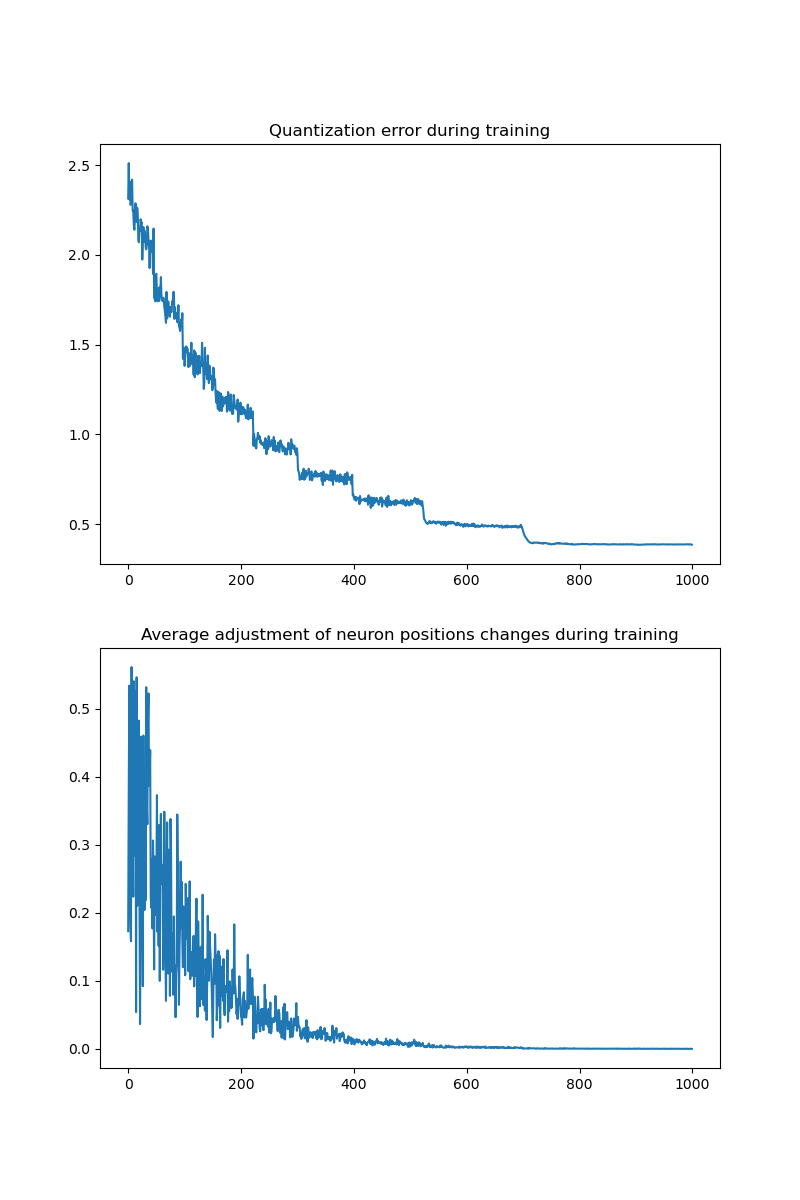
\includegraphics[width=0.95\textwidth]{../errors.png}
		\caption{Quantizačnej chyby a priemernej zmeny pozície neurónu počas trénovania modelu }
	\end{figure}
	
	Vidíme, že quantizačná chyba klesá pomerne skokovo keď určitý počet epoch sa chyba mení minimálne a náhle v jednej epoche klesne výraznejšie. Finálna chyba je približne $0.375$. V prípade priemernej zmeny pozície neutrónov vidíme, že postupne klesá a po približne 600 epochách je iba minimálna.
	\\
	
	Keď si pozrieme ktoré neuróny aktivujú jednotlivé triedy dostaneme takýto výsledok:
	
	\begin{figure}[!h]
		\centering
		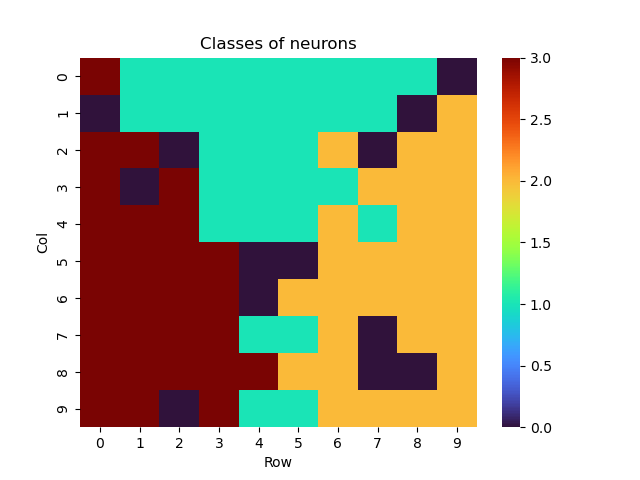
\includegraphics[width=0.95\textwidth]{../class_neur.png}
		\caption{Triedy aktivujúce jednotlivé neuróny}
	\end{figure}
	
	Vidíme, že na hraniciach medzi triedami ostalo niekoľko neurónov ktoré nie sú aktivované žiadnou triedou ale inak vidíme pomerne pekné hranice jednotlivých tried (výnimkou je pár neurónov klasifikovaných ako trieda 1 na hranici tried 2 a 3).
	\\
	
	Na základe tohto výsledku sa môžeme pokúsiť klasifikovať našu testovaciu množinu vstupov. Pri porovnaní predikcii modelu a skutočných tried sme zistili, že náš model klasifikoval správne $81.7\%$ testovacích bodov. Pričom rozdelenie tried správne klasifikovaných bodov bolo následovné: $\{1: 13,\quad 2: 14,\quad 3: 22\}$. Čiže najhoršie výsledky dosiahol pre triedu 1 kde správne klasifikoval iba približne $68\%$ bodov, o niečo lepšia bola trieda 2 kde správne klasifikoval takmer $78\%$ a úplne najlepšou bola trieda 3 kde bolo správne klasifikovaných až vyše $95\%$ bodov. Ak si pozrieme celú confusion matrix zistíme, že veľká časť chýb je spôsobená tým, že testovací vstup skončí v mŕtvom neuróne:
	
	\begin{table}[!h]
\begin{tabular}{|p{0.2\textwidth}|p{0.08\textwidth}|p{0.08\textwidth}|p{0.08\textwidth}|p{0.08\textwidth}|}
\hline
očakávanie/realita& 1& 2& 3& 0\\ \hline
1 & 68.42\% & 0.0\% & 15.79\% & 15.79\% \\ \hline
2 & 5.56\% & 77.78\% & 0.0\% & 16.67\% \\ \hline
3 & 0.0\% & 0.0\% & 95.65\% & 4.35\% \\ \hline
\end{tabular}
\end{table}

	\newpage
	
	Ako ďalšie si môžeme pozrieť heatmapy pre jednotlivé parametre modelu (máme ich 7):
	
	\begin{figure}[!h]
		\centering
		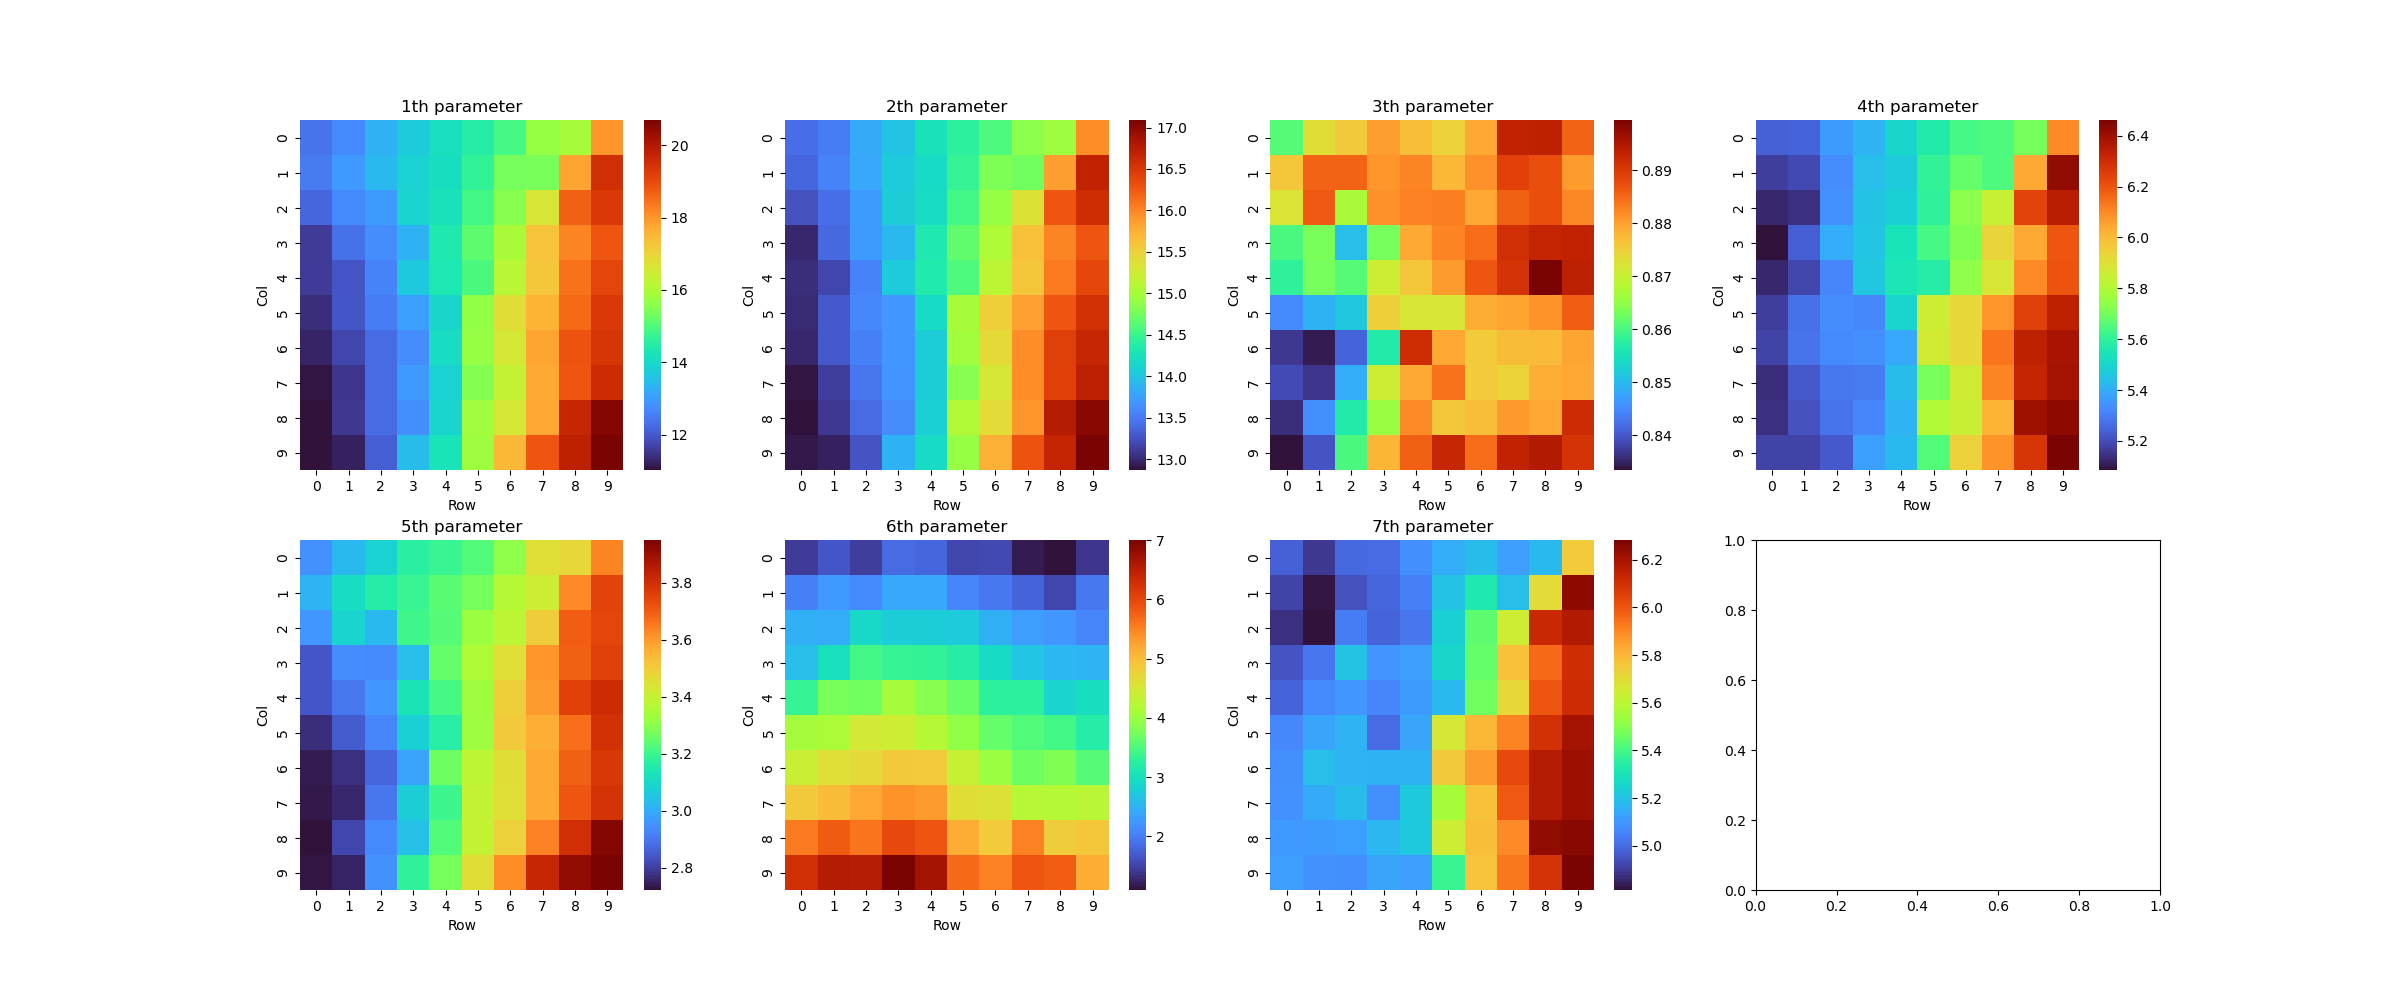
\includegraphics[width=0.7\textwidth]{../param_heatmaps.png}
		\caption{Heatmapy jednotlivých parametrov modelu}
	\end{figure}

	Na týchto heatmapách si môžeme všimnúť, že pre parametre 1, 2 a 5 vyzerajú takmer totožne a pre parametre 4 a 7 sú veľmi podobné pričom podobnosť je aj s rozdelením tried (na grafe vyššie). Heatmapy pre parametre 3 a 6 sú diametrálne odlišné od ostatných aj navzájom.
	\\
	
	Na záver si ešte vizualizujme U-matrix pre našu SOM:
	
	\begin{figure}[!h]
		\centering
		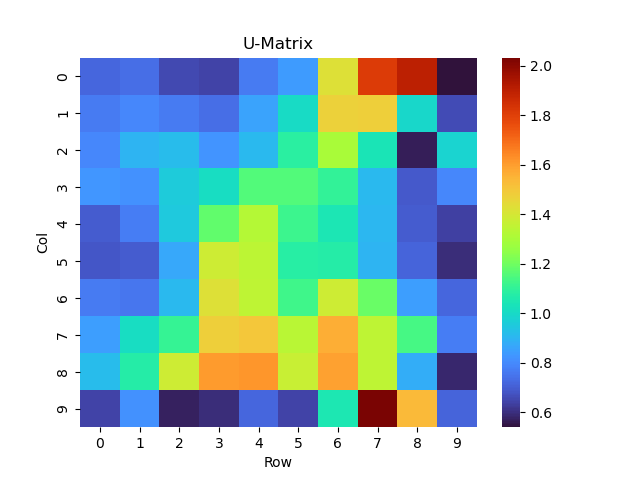
\includegraphics[width=\textwidth]{../u_matrix.png}
		\caption{U-matrix}
	\end{figure}

	Úprimne, si nie som istý ako tento výsledok interpretovať, teoreticky by mal znamenať, že model našiel 2 (teoreticky 3) clustre dát, jeden vidíme hore v pravom rohu a druhý dole v strede matice (teoreticky tretí dole v pravom rohu). Avšak tento výsledok je výrazne odlišný od výsledku tried pre jednotlivé neuróny, čo by mohlo indikovať zle natrénovanú sieť, avšak v takom prípade by sme nepredpokladali tak vysokú presnosť zaradzovania do tried ($>80\%$).  
	  
\end{document}